% -*- latex -*-
%%%%%%%%%%%%%%%%%%%%%%%%%%%%%%%%%%%%%%%%%%%%%%%%%%%%%%%%%%%%%%%%
%%%%%%%%%%%%%%%%%%%%%%%%%%%%%%%%%%%%%%%%%%%%%%%%%%%%%%%%%%%%%%%%
%%%%
%%%% This text file is part of the theory writeup on the
%%%% Integrative Model for Parallelism,
%%%% copyright Victor Eijkhout (eijkhout@tacc.utexas.edu) 2014-6
%%%%
%%%% eager.tex : master file for report IMP-19
%%%%
%%%%%%%%%%%%%%%%%%%%%%%%%%%%%%%%%%%%%%%%%%%%%%%%%%%%%%%%%%%%%%%%
%%%%%%%%%%%%%%%%%%%%%%%%%%%%%%%%%%%%%%%%%%%%%%%%%%%%%%%%%%%%%%%%
\documentclass[11pt,fleqn,preprint]{impreport}

\taccreportnumber{IMP-19}

\input setup

\title[IMP progress 2014/15]{Progress report on the Integrative Model\\ under NSF EAGER grant 1451204}
\author[Eijkhout]{Victor Eijkhout\thanks{{\tt
      eijkhout@tacc.utexas.edu}, Texas Advanced Computing Center, The
    University of Texas at Austin}}

\begin{document}
\maketitle

\begin{abstract}
  The Integrative Model for Parallelism (IMP) is a parallel programming
  system, primarily aimed at scientific applications.

  Its aim is to offer an integrated model for programming many
  different modes of parallelism. In fact, in the IMP system one
  source file can be compiled into message passing, \acl{DAG}-based,
  and hybrid execution models. Also, performance enhancing techniques
  such as redundant computation and latency hiding are automatically
  achieved without need for programmer intervention.

  From September 2014 through August 2015 the IMP project
  was supported by NSF Eager grant 1451204. We report on
  progress made during that time.
\end{abstract}

\acresetall

\section{The Integrative Model for Parallelism}

The Integrative Model for Parallelism (IMP) is a parallel programming
system based on a new theory of parallel computing,
primarily aimed at scientific applications.

By offering a mathematical description of distributed objects
and calculations, IMP arrives at a description of parallel algorithms
that is independent of the actual type of parallelism. 
Thus, we can compile one source file into MPI, \ac{DAG}-based
(such as OpenMP tasking), and hybrid
execution models. The theory is powerful enough to formalize techniques
such as redundant computation and latency hiding.
The IMP sytem can apply such optimizations achieved without
need for programmer intervention.

Proof-of-concept tests show a performance similar to code written
by hand or realized in popular libraries such as PETSc.

\subsection{IMP API basics}

To the user, the IMP software
offers an interface that can be described as `sequential programming
with distributed objects'. The basic sequential step is called a~`kernel',
and it corresponds to a generalized notion of a data parallel operation:
an operation that takes one or more distributed objects as input,
and produces a distributed object as output, where each element of the output
can be computed independently.

\begin{figure}[ht]
  \includegraphics[scale=.1]{imp_structure}
  \caption{Structure of the IMP system}
  \label{fig:structure}
\end{figure}

The IMP system then translates this user description of an algorithm to an
\ac{IR} that is independent of the underlying mode of parallelism.
A~second translation stage then realizes this as a parallel program
in a particular system, for instance using
MPI or OpenMP calls\footnote {We use the tasking mechanism
  of OpenMP, not the more common loop parallelization functionality.}
or hybrid combinations.

\subsection{Inspector-executor} To the user an IMP program looks like
a sequential program of C++ library calls. However, instead of being executed,
these library calls actually insert a kernel (see above)
into a algorithm data structure. This algorithm
is then separately analyzed and executed, in a clear case of the inspector-executor
paradigm~\cite{Sussman92partiprimitives}. A~first result of the algorithm
analysis is a kernel dataflow formulation
based on a dependency analysis of the input and output objects.
A~task dataflow graph as it is commonly considered is then derived
by considering the execution of a kernel on a processing element as a task.

\subsection{Dataflow}
\label{sec:dataflow}

The previous item mentioned two forms of dataflow.
An example will elucidate this distinction.

The heat equation
is rendered by a single sequence of kernels; see figure~\ref{fig:heat-flow}, left.
This is the dataflow that the user programs.
%
On the other hand, the task dataflow that governs interaction between
processors is derived by the IMP system; see figure~\ref{fig:heat-flow} right.

Thus our notion of dataflow programming is much simpler
than dataflow programming as it is commonly proposed. In essence,
the programmer codes the algorithm, not its execution.

\begin{figure}[p]
\hbox\bgroup
  \includegraphics[scale=.4]{heat-kernels}
  \includegraphics[scale=.4]{heat-tasks}
  \egroup
  \caption{Kernel dataflow (left) and task dataflow (right) for the one-dimensional heat equation,
    executing 15 steps on 6 processors.}
  \label{fig:heat-flow}
\end{figure}

\subsection{Communication and synchronization}

Based on the kernel dataflow graph and distribution of objects
specified by the programmer, the IMP system derives a
(much larger) task dataflow graph.
The task dependencies can be satisfied as MPI messages,
or as OpenMP explicit task directives.

We note that we do not concern ourselves with the task-local code,
which is provided through a function pointer, much as in other
\ac{DAG} execution models such as Quark~\cite{Yarkhan:quark-report}.
This may be a question for a compiler project in the future; see
section~\ref{sec:local}.

\section{Work performed}

In the past year, we have solidified the IMP infrastructure,
written the MPI and OpenMP backends to where they can implement
some meaningful codes, and have started on the MPI+OpenMP hybrid
backend.

\subsection{Infrastructure; MPI and OpenMP backends}

We have proved the integrative nature of our model by realizing both a
message passing (MPI) and DAG-based (OpenMP) backend to our software.
This required building a substantial amount of
infrastructure. Interesting is the generalization of the communication
and synchronization mechanisms and the  algorithm execution.

Also we implemented a very crude sparse matrix class. Under the assumption that
for many sparse matrices bandwidth is the performance determining factor,
we did not optimize this at all.

As an indication of our conceptual integration in code, we mention that
the base code is around 4k lines, with 1.5k lines for
the derived classes of MPI and OpenMP each,
and 0.7k lines for MPI/OpenMP hybrid. (We also note that our testing
code is about 16k lines, double that of all the actual library code.)
About half of this codebase is written in the past year.

\subsection{Hybrid computing}
\label{sec:hybrid}

In probably our most intriguing development, we have combined the MPI
and OpenMP backends, and combined them into a hybrid MPI+DAG implementation.
(As noted above, thanks to our fargoing code reuse design, this
part of the library is actually very small.)
In our current design, we take MPI communication and synchronization
mechanisms, but replace the 
task-local code by an OpenMP \ac{DAG} of tasks.

This serves several purposes. For instance, on very large processor counts
it cuts down on the $O(P)$ space that is typically allocated on each
process. In case of irregular workloads it can also achieve a statistical
load balancing by making load-to-processor assignment flexible.

However, the main promise of hybrid computing lies in the future; see
section~\ref{sec:future-hybrid}.

\subsection{Conjugate gradients}

Using a crude sparse matrix class we implemented a conjugate gradients
method, and compared its performance to a PETSc code. We see that our
code is slower than PETSc, but by less than a factor of~2. More
importantly, we note that our scaling behaviour looks similar to
PETSc\footnote {At the moment, scaling to large numbers of processors
  runs into a design mistake: we wanted each messsage to be
  identifiable by a unique tag. Unfortunately MPI tag space is not
  large enough for this.  This will be fixed fairly quickly.}.

\begin{wrapfigure}{r}{2.3in}
  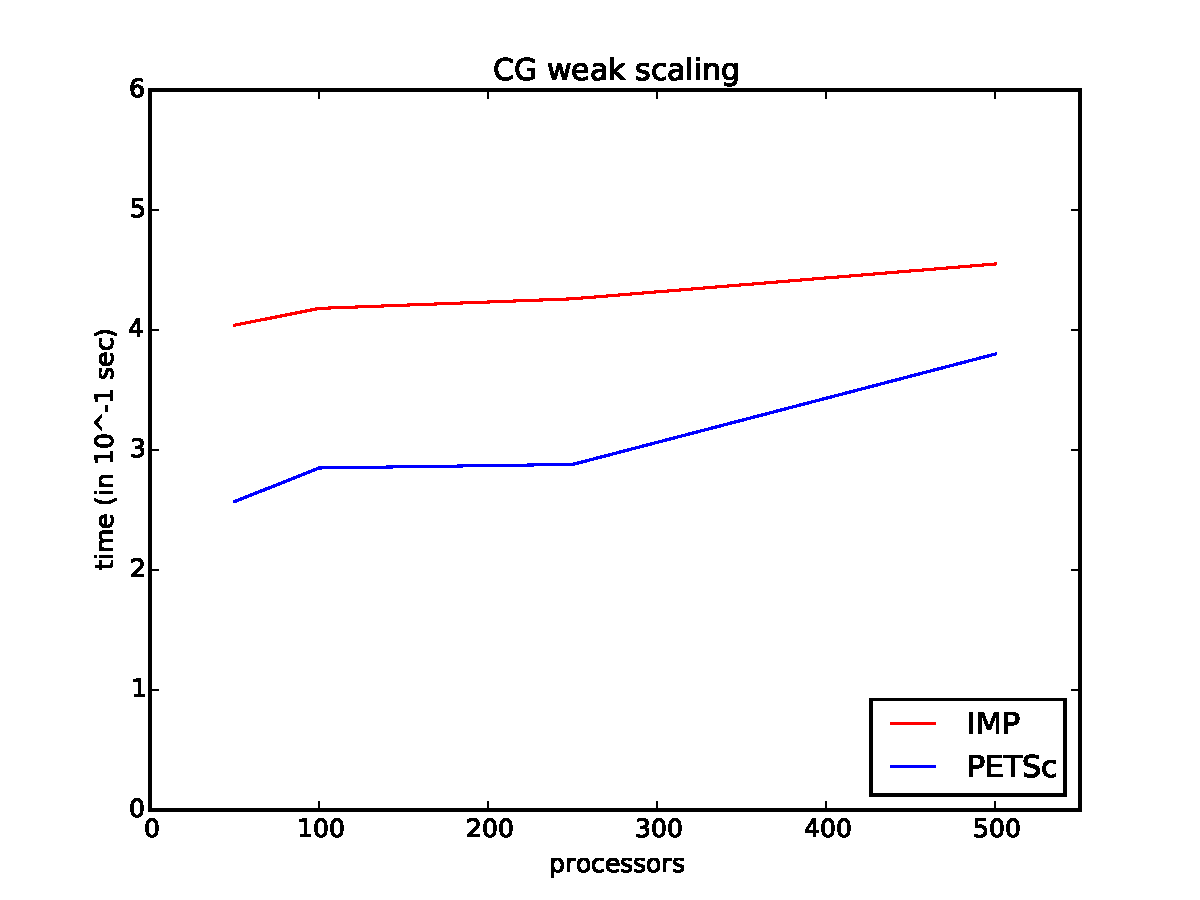
\includegraphics[scale=.3]{cg_mpi_scaling}
\end{wrapfigure}
%
Our CG code (see figure~\ref{fig:cgtemplate})
%
\begin{figure}[p]
\verbatimsnippet{cgtemplate}
  \caption{Loop body of the IMP CG code}
  \label{fig:cgtemplate}
\end{figure}
%
looks in fact much like the PETSc implementation, with one
library call per basic linear algebra operation (inner product, matrix-vector
product, et cetera). Two differences: first of all, these linear algebra operations
are themselves implemented in IMP, as opposed to the PETSc operations which can
be low level code. Secondly, IMP code looks slightly more intricate, since scalar operations
are operations on redundantly distributed objects, and therefore have to be realized
with library calls.

\subsection{N-body problems}
\label{sec:nbody}

We have implemented the algorithm structure of a tree code such as for an N-body problem;
see~\cite{Salmon86fastparallel}. 
Figure~\ref{fig:nbody-kernels} shows the resulting kernel dataflow.
(See section~\ref{sec:dataflow} for a discussion of dataflow in the IMP model.)

\begin{figure}[p]
  \includegraphics[scale=.2]{nbody-kernels}
  \caption{The kernel structure of an N-body code}
  \label{fig:nbody-kernels}
\end{figure}

%% \begin{figure}[p]
%%   \includegraphics[scale=.2]{nbody-tasks}
%%   \caption{The task structure of an N-body code}
%%   \label{fig:nbody-tasks}
%% \end{figure}

The point of interest in this application is the treatment of the
higher tree levels, where there are fewer points than
processors. Since IMP takes a very symmetric look at processes, it
uses redundant replication of points on these levels.
The decision to use replication can be defended from a point of energy efficiency.
Under this strategy the prolongation down the tree is fully local, whereas
a non-replicated strategy would involve a good deal of message traffic.

The resulting
algorithm is illustrated, for 8~leave nodes and 4~processors, in
figure~\ref{fig:uptree}.

\begin{figure}[ht]
  \includegraphics[scale=.17]{nbody-8421}
  \caption{Computation and communication up the tree}
  \label{fig:uptree}
\end{figure}

The main point worth noting here
is that this takes no effort at all to program: the user never specifies the redundancy, only
the halving of the points per level. In the following code snippet the distribution
\n{level_dist} on the finest level is given; all other distributions, including the redundantly
replicated ones, are derived here:

\verbatimsnippet{uptreelevels}

\subsection{Latency optimization}

MPI non-blocking calls hold the promise of overlapping computation and communication.
To this end, the IMP system moves posting the Isend and Irecv calls as far down the task
graph as possible. This also implies that non-blocking collectives can be employed
in the IMP system without the user ever having to specify them.

On our current test systems, this mechanism has not paid off by more than a modest 10--15
percent. We will seek out clusters that offer hardware support for communication offload.

\section{Future work}

\subsection{Latency tolerance and communication avoidance}
\label{sec:future-hybrid}

Probably the most exciting future prospect of our hybrid scheme of section~\ref{sec:hybrid}
is manipulations on the global task graph. If each MPI-task contains a non-trivial OpenMP
task \ac{DAG}, we can migrate and duplicate tasks between MPI processes in such
a way as to effect a `communication avoiding' scheme~\cite{Demmel2008IEEE:avoiding}.

In \impref{06} we formally derived the task subsets that will completely hide
latency, while minimizing communication and redundant computation. 

\begin{figure}[ht]
  \includegraphics[scale=.1]{div-avoid}
  \caption{Formal derivation of a communication avoiding partitioning of a task graph}
  \label{fig:avoid}
\end{figure}

\subsection{Local code generation}
\label{sec:local}

In the current IMP design, the task-local code is provided by a function pointer.
The local code is different between MPI and OpenMP, and perhaps even between standalone OpenMP
and OpenMP in hybrid context. Generation of this code from a more abstract description of the
algorithm is an open question.

While the mere generation of this code is only a moderately interesting project,
various other questions have research potential:
\begin{itemize}
\item Can code be generated with annotations on where it synchronizes with other tasks,
  and where it is independent? Can the synchronization be quantified? As argued elsewhere,
  this may lead to programmable prefetch streams, which can obviate caches and coherence.
\item If we go to very fine-grained tasks, can a compiler generate code that optimally
  uses registers and last-level caches?
\item Can code generation interact with an optimization mechanism, so that granularity
  is adaptively chosen?
\end{itemize}

\subsection{The Eijkhout-McCalpin garbage preventor}
\label{sec:garbage}

The above description of kernel dataflow being based on input and output objects
implicitly carries the assumption that an object is only ever created once,
reminiscent of a functional programming style.
However, the dynamic memory management and attendant garbage collection
are unacceptable in a scientific computing context. Therefore we can indicate
that one object reuses the memory of another.

The typically application for this mechanism is an iterative loop, where
each iteration produces a new object, but based on the memory of the object
of the previous iteration. In many cases, the user can make the decision to
reuse; however, we have a theoretical framework under which the system can
make such a decision; see~\impref{04}.

\subsection{Distributions}

Our distribution mechanism is theoretically clear. Practical implementation
is a matter of time. The following two directions are considered
for future work.

Implementing dense linear algebra would be an interesting test case
for the IMP model. For this we first of all need to develop
two-dimensional distributions.

All of our test applications at the moment have a very symmetrical
treatment of the processes. Locally adaptive grid refinement
can be formulated in the IMP theory by using partially defined
distributions. The theory for this, and some mathematically described
examples, are found in~\impref{01}. The implementation is another story.

\subsection{Redundant work and other resiliency topics}

IMP distributions easily accomodate redundant computation as we have
shown in simple examples. However, we have not yet implemented redundant
duplication of whole tasks. While the model supports this, the implementation
needs much research.

Communication avoidance (see~\ref{sec:future-hybrid} above) is one application
of this mechanism; another would be adding resilience to the model.
Rather than pure duplication, we could also consider the on-demand recomputation
of failed tasks.

\section{Conclusion}

We have shown in a proof-of-concept code that it is possible to code
scientific applications in an essentially sequential manner,
with the translation to multiple parallel backends happening
automatically. The translating stage is smart enough to reproduce
the performance of traditional codes; non-trivial code transformations
are a distinct future possibility.

\subsection*{Acknowledgement}
\input ack

\bibliography{vle}
\bibliographystyle{plain}

\end{document}
